\documentclass[11pt]{article}
\usepackage{acl2013}
\usepackage{times}
\usepackage{latexsym}
\usepackage{amsmath}
\usepackage{amsfonts}
\usepackage{multirow}
\usepackage{url}
\usepackage{xspace}
\usepackage{verbatim}
\usepackage{algorithm2e}
\usepackage[retainorgcmds]{IEEEtrantools}
\DeclareMathOperator*{\argmax}{arg\,max}
\DeclareMathOperator*{\argmin}{arg\,min}

\usepackage{color}
\usepackage[pdftex]{graphicx}
\usepackage{caption}
\usepackage{subcaption}
\usepackage{multirow}

\numberwithin{equation}{section}

\setlength\titlebox{6.5cm}    % Expanding the titlebox

\title{Bag-of-Phrases Machine Translation}

\author{Waleed Ammar \and Manaal Faruqui\\
  Language Technologies Institute \\
  Carnegie Mellon University \\
  Pittsburgh, PA, 15213, USA \\
  {\tt \{wammar, mfaruqui\}@cs.cmu.edu} 
}
\date{}
%\author{}

\begin{document}
\maketitle
\begin{abstract}
	
We present a novel bag-of-phrases based machine translation model which attempts to reduce the
computational complexity as well as the space complexity of a standard phrase-nased translation
system. We propose to decompose the sentence translation problem into two independent components: (a) 
bag-of-phrase translation (b) phrase reordering. We then tune our bag-of-phrase translation system using PRO and report results.
\end{abstract}

\section{Introduction}
Statistical machine translation (SMT) is a well research area that encompasses various ways of machine translation (MT)
like phrase-based MT~\cite{Koehn:2003:SPT:1073445.1073462} and hierarchical phrase-based MT~\cite{Chiang:2007:HPT:1268656.1268659}.
These approaches to machine translation are the current state-of-the-art and are heavily used. Both of these approaches
attempt to solve the problem of translation phrases in the source sentence to the target language and the reordering
of these phrases in the target at the same time. This leads to an explosion of the hypothesis space and quickly
even for very small sentences becomes computationally intractable. This effect is shown in Figure~\ref{fig:exp-hyp}. Such an explosion
of the hpothesis space can lead to potential errors in decoding.

In particular, a sentence of length $n$, can be segmented in $2n$ ways. Assuming each source phrase can be translated in $l$ ways, for each source sentence segmentation of $s$ phrases, there are a maximum of $l^s \times s!$ complete sentence translation hypotheses.
Various heuristics have been used to prune the hypothesis space by taking the $k$-best hypothesis at every step of the stack decoding.
Different type of scores can be used to evaluate a partially translated hypothesis, usually a future cost is added to the hypothesis 
which measures what is the best score that this hypothesis can achieve. Based on these scores, the stack of possible hypothesis can
be pruned but all these are heuristics which might not be accurate.

We aim to reduce the hypothesis space of the translations without using heuristics measures. This can only be achieved if instead
of pruning the hypothesis space we break down the translation process into two separate processes: \textit{phrase translation} \& 
\textit{reordering}. We call such an approach to MT \textit{bag-of-phrases machine translation}. Using bag-of-phrase translation reduces the complete hypotheses count for each segmentation of $s$ phrases into $l^s$ from $l^s \times s!$ which, although exponential in $s$, is a much smaller space.

\begin{figure*}[t]
  \centering
  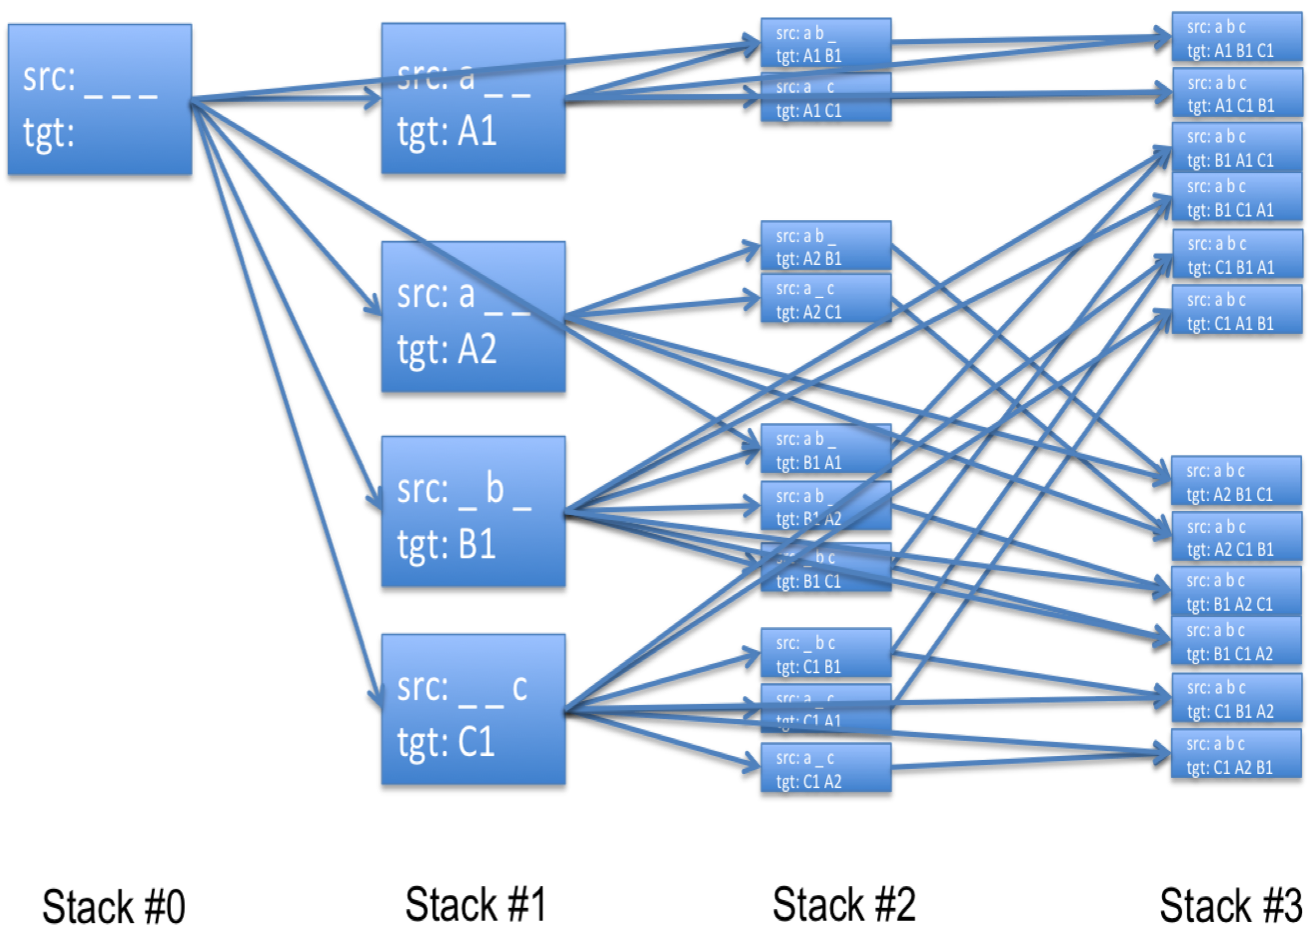
\includegraphics[width=1.5\columnwidth]{hyp-explosion.png}
  \caption{Explosion of hypothesis space in Phrase-based MT}
  \label{fig:exp-hyp}
\end{figure*}

\section{Bag-of-phrase Translation}
\label{sec:bof}

The first step in our translation is translating the source phrases into target language.
This can further be broken down into two units: (a) splitting the source sentence into phrases,
(b) translation of sources phrases.

We execute these two steps together at the same time using CYK parsing~\footnote{\url{http://en.wikipedia.org/wiki/CYK_algorithm}}.
For every sentence in the source language, we construct a CYK table where we fill every node in the table using the phrases
from the translation model. We start with the bottom most nodes where every node just contains the words in the source sentence
and incrementally move up in the chart by trying to merge two words or two phrases together by checking if they are present in the
translation model. For every entry of a possible phrase in a given node of the chart we also include its translation in the 
target language which again is obtained from the phrase table of the translation model. This is our basic translation step in the 
bag-of-phrases translation model.

We further augment this step by including various filters at every node to ensure that only the best translation of the phrases appear
on the final node. Each of our phrase translation has a translation model scores by default. We incorporate some other scores
to make a more informed decisions while selecting which phrases should be pruned out in every node. We include the following more
scores for every phrase translation: (a) The DWL score (cf. section~\ref{sec:dwl}) (b) The unigram LM score. We have weights for each 
such feature and we keep the $k$-best phrase translations at every node. Further details will be discussed in 
section~\ref{sec:experiments}.

We also face the problem of duplicate entries in our CKY table nodes. As we know, in CKY a node can contain multiples phrases which 
come from different lower level nodes. Many of these phrases are duplicaed of each other as our phrase combination step is associative.
For example, a phrase ``i love you'' can be formed by concatenation ``i'' \& ``love you'' or ``i love'' \& ``you''. We formulate a hash
function which is able to identify all such duplicate pairs and eliminate them.



\begin{figure*}[tb]
  \centering
  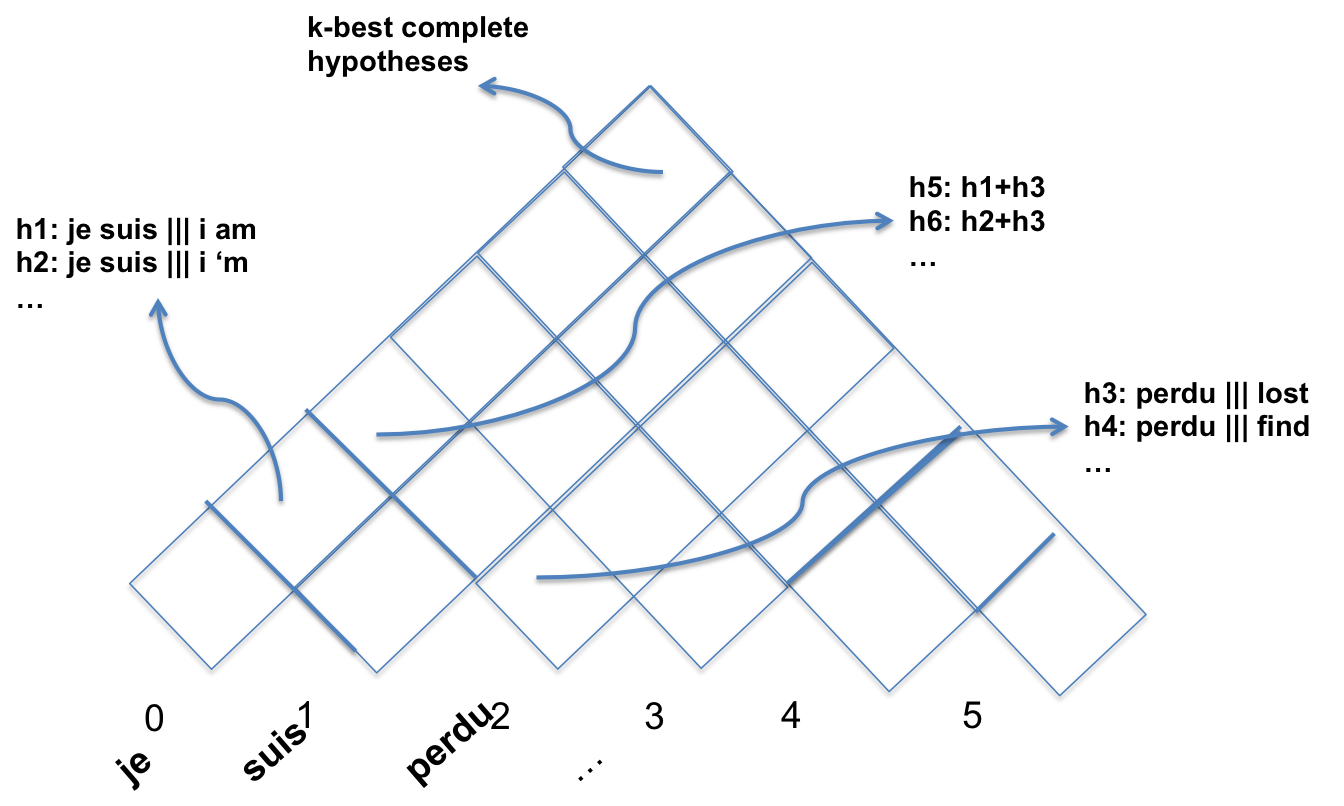
\includegraphics[width=1.5\columnwidth]{cky.png}
  \caption{Bag-of-phrase translation using CYK parsing}
  \label{fig:cky}
\end{figure*}

\section{Phrase Reordering}
\label{sec:reordering}

Given a bag-of-phrases translation we need to arrange the phrases in the bag to find the translated
sentence. For a bag-of-phrases containing $k$ phrases, $k!$ different arrangements of the phrases is
possible. This is exponential in the size of the bag and is computationally intractable. We thus
resort to dynamic programming approach using finite state automaton (FSA).

\subsection{Construction of the FSA} 
Suppose we use an $n$-gram language model. Then the probability
of occurrence of the a word in the sentence depends on the previous $n-1$ words in the sentence. Thus,
for every word we need to know the previous $n-1$ words while computing its score. We construct an
automaton that has $k$ ($k$ = no. of phrases) different layers symbolizing the no. of phrases rearranged
till that point. We calculate the possible no. of unique $(n-1)$-grams that can result from different arrangements
of the phrases. If the length of a given phrase is greater than $n$ then we also include the $n$-grams inside
the phrase in the set. Let the total no. of possible $n$-grams be $g$. For every layer in the FSA we now construct
$g$ states. We finally add a statr state and a final state to the automaton.

Every transition in the automaton starts from a state which represents an $(n-1)$-gram consumes a given phrase
with the probability of observing that phrase (language model score) given the previous $(n-1)$-gram and goes to the next state which 
represents new $(n-1)$-gram. From the initial state we have transitions for all possible phrases to the first layer
and from the first layer we have transitions from all states for all possible phrases to the next layer and so on.
Finally, from all the states in the final layer we have a special token $\langle/s\rangle$ that marks the end of the sentence
and has the probability of observing the previous $(n-1)$-gram at the end of the sentence. Figure~\ref{fig:reordering} shows an automaton constructed for the reordering of phrases \{``i am'', ``lost'', ``.'' \}.

\begin{figure*}[t]
  \centering
  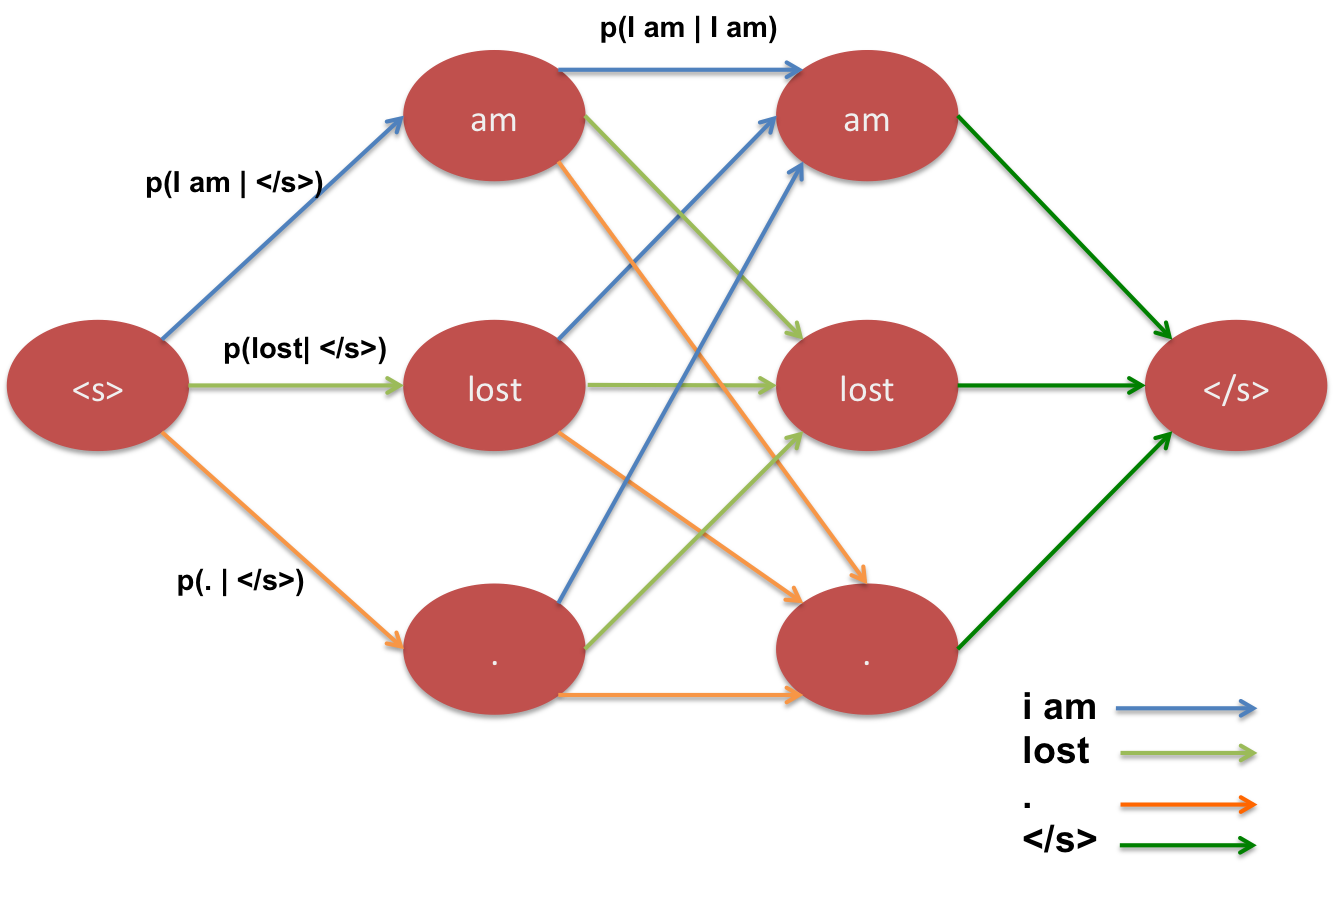
\includegraphics[width=1.5\columnwidth]{reordering.png}
  \caption{FSA constructed for reordering a given list of phrases using a unigram LM.}
  \label{fig:reordering}
\end{figure*}

\paragraph{Computing the best reordering}
The FSA now represents a lattice where every path from the initial state to the final state is a possible reordering of
the sentence. However, not all the enumeration of the paths are valid paths because the paths may contain repitition of phrases.
The reason this could happen is because of the fact that our automaton doesn't store the entire history in its states, it only
knows the previous $(n-1)$-gram of the sentence being formed. Hence, there are edges in the automaton which are reusing the 
phrases.

We defined a new semiring to avoid this problem. For every arc of the automaton, along with the language model score we also included
a bit vector which represents the phrase being currently consumed in the transition. So, every element of our semiring looks like this:
\[
(lm, [0,0,0,1,0, \dots 0, 0])
\]
where, \textit{lm} represents the language model score and the $1$ at the fourth position represents that the fourth phrase is being consumed in this particular transition.

We define the $\otimes$ operation on this semiring as follows:

if $bv1 \cap bv2 = [0,0, \dots 0]$ :
\[
(lm1, bv1) \otimes (lm2, bv2) = (lm1 \times lm2, bv1 \vert bv2) \\
\]
else if $bv1 \cap bv2 \neq [0,0, \dots 0]$ :
\[
(lm1, bv1) \otimes (lm2, bv2) = (-\infty, bv1 \vert bv2) 
\]

We define the $\oplus$ operation on this semiring as follows:
if $lm1 > lm2$:
\[
(lm1, bv1) \oplus (lm2, bv2) = (lm1, bv1) \\
\]
else:
\[
(lm1, bv1) \oplus (lm2, bv2) = (lm2, bv2) \\
\]

Thus, the $\oplus$ operator selects the best path till a given state and the $\otimes$ operator computes
the score of the path and also maintains the bit-vector of the phrases used till now. If a phrase
is recurring on a path then the semiring gives it a very low score ($-\infty$) and hence that path is effectively
removed from the posssible orderings. Now, having defined the semiring we compute a list of best paths according to the language model 
score and output it.
Our automata were designed usig Openfst toolkit\footnote{\url{www.openfst.org}}~\cite{openfst}. We used the 
Pyfst\footnote{\url{https://github.com/vchahun/pyfst}} interface to access Openfst through python.

\section{Reranking}
\label{sec:reranking}

We have implemented Pairwise Ranking Optimization (PRO)~\cite{hopkins-may:2011:EMNLP} method for reranking our translated $k$-best 
output lists. PRO has the advantage of being able to tune a large number of parameters over other tuning methods like MERT~\cite{Och:2003:MER:1075096.1075117}. Each of our $k$-best lists is augmented with the following feature values:-

\paragraph{$p(t|s)$ :} The probability of observing the target given the source sentence.
\paragraph{$p(s|t)$ :} The probability of observing the source given the target sentence.
\paragraph{$p_{lex}(t|s)$ :} The lexical probability of the target given the source sentence.
\paragraph{$p_{lex}(s|t)$ :} The lexical probability of the source given the target sentence.
\paragraph{$p_{dwl}(t|s)$ :} The probability of observing words given in the target sentence given the source according to a discriminative word lexicon (DWL) (discribed later).
\paragraph{$n_{dwl}(OOV)$ :} The number of out of vocabulary words in the target sentence according to the DWL.
\paragraph{$len(t)$ :} The length of the target sentence.
\paragraph{$n_{rep}(t)$ :} The number of repititive tokens in the target. Some of the special symbols (ex. punctuation markers) have been allowed to repeat.
\paragraph{$p_{lm}(t)$ :} The probability of observing the target sentence according to a unigram language model.

We sample a total to $5000$ sentence pairs from the $k$-best output list and then take the top 50 sentence pairs according to the
difference in their BLEU~\cite{Papineni:2002:BMA:1073083.1073135} scores. We do this in order to make the tuning faster as opposed to 
sampling $5000$ sentence pairs for every source sentence. We then train a Logistic Regression classifier to find weights for the
various features described above. Once we have the weights for the features, for every sentence in the $k$-best list we evaluate the 
probability of it being a better translation and the sentence with the highest probability is selected as our output translation 
sentence.

\subsection{Discriminative Word Lexicon}
\label{sec:dwl}

Discriminative models have been shown to outperform generative models on many natural language processing tasks. For machine 
translation, however, the adaptation of these methods is difficult due to the large space of possible translations and the size of the 
training data that has to be used to achieve significant improvements. 

We implement a discriminative word lexicon as described in~\cite{Mauser:2009:ESM:1699510.1699538}.
The core of the model is a classifier that predicts target words, given the words of the source
sentence. The structure of source as well as target sentence is neglected in this model. We do
not make any assumptions about the location of the words in the sentence.

We model the probability of the set of target
words in a sentence $t$ given the set of source words
$s$. For each word in the target vocabulary, we can
calculate a probability for being or not being included in the set. The probability of the whole set
then is the product over the entire target vocabulary $t$:
\[
p_{dwl}(t|s) = \prod_{t_i \in t} p(t_i|s) \prod_{t_j \in V-t} p(t_j|s)
\]

The discriminative word lexicon model has the
convenient property that we can train a separate
model for each target word making parallelization straightforward.
For every word in the target vocabulary we train a Logistic Regression classifier with L2 regularization.
Every sentecne in the training data is a training instance for the DWL of a given word.

\section{Related Work}
\label{sec:relatedWork}

\section{Experiments}
\label{sec:experiments}

Since, we did not have sufficient time to evaluate both parts of our translation approach we decide to evaluate
the performance of our \textit{phrase translation} step. The performance of the reordering stage is dependent
on the translation step and hence its important to make sure that the first step is working fine.

For this, we implemented an \textit{oracle} reordering algorithm which returns the rearragement of the phrases
which results in the maximum BLEU score one can achieve for a given reference translation.


\section{Conclusions}
\label{sec:conclusions}

\section{Future Work}

Though our reordering model seems exact for a given $n$-gram model, it is not so. The way we define the $\oplus$ operator
in our semiring allows us to compare two partially constructed hypotheses which have translated different source phrases
and are hence not stricly comparable. Thus, with the score of the partially translated hypotheses we could also include
the future cost\footnote{\url{http://homepages.inf.ed.ac.uk/pkoehn/publications/tutorial2006.pdf}} of the translation which would help 
us make a more informed decision.

Although we want to keep the translation part and the reordering part separate from each other, we expect that including the language 
model score in the final score during the decoding could actually help obtain better phrases.

\bibliography{references.bib}
\bibliographystyle{naaclhlt2013}
\end{document}
